\chapter{Pruebas Experimentales y Resultados}
\label{chap:pruebas}

En este capítulo se recogen los ensayos experimentales llevados a cabo tanto a nivel de emulación en software (\textit{Software-in-the-Loop}, SIL) como en la comunicación física sobre hardware (\textit{Hardware-in-the-Loop}, HIL).

\section{Evaluación del rendimiento computacional (Benchmark C++20 vs Python)}
\label{sec:benchmark_rendimiento}

Para cuantificar objetivamente la ganancia de rendimiento obtenida tras la reingeniería del driver, se ejecutó un banco de pruebas comparativo de 1.000.000 de operaciones consecutivas frente a la librería original en Python (\texttt{xgolib\_dog.py}) suministrada por el fabricante.

Los resultados empíricos obtenidos se detallan en la Tabla~\ref{tab:benchmark_driver}.

\begin{table}[htbp]
    \centering
    \caption{Comparativa de rendimiento entre la librería original Python y el nuevo driver C++20 (1.000.000 operaciones).}
    \label{tab:benchmark_driver}
    \begin{tabular}{lccc}
        \toprule
        \textbf{Operación evaluada} & \textbf{Python (\texttt{xgolib\_dog})} & \textbf{C++20 (\texttt{xgo\_driver})} & \textbf{Aceleración (\textit{Speedup})} \\
        \midrule
        Mapeo físico y creación trama TX & 440.74\,ms & 30.06\,ms & \textbf{14.6$\times$} \\
        Desempaquetado flotante (\texttt{Byte2float}) & 285.68\,ms & 0.84\,ms & \textbf{340$\times$} \\
        Parseo de flujo UART RX (900.000 bytes) & 54.29\,ms & 7.17\,ms & \textbf{7.6$\times$} \\
        \midrule
        \textbf{Tiempo total de ejecución} & \textbf{780.71\,ms} & \textbf{38.08\,ms} & \textbf{20.5$\times$ más rápido} \\
        \bottomrule
    \end{tabular}
\end{table}

Como se observa, el nuevo controlador reduce el tiempo total de procesamiento en más de un 95\%, con una mejora crítica en el desempaquetado numérico de telemetría de 340 veces, liberando capacidad computacional esencial en la Raspberry Pi CM5.

\section{Validación en hardware físico real}
\label{sec:validacion_hw}

Se ha verificado experimentalmente el enlace serie bidireccional entre la Raspberry Pi CM5 y la placa controladora de los cuadrúpedos a través de \texttt{/dev/ttyAMA0}. Las pruebas confirman la recepción continua de la IMU y la odometría de los servomotores a 115200 baudios, así como la actuación correcta del mecanismo de parada por timeout del watchdog.

\section{Validación en simulación (SIL) sobre Gazebo Harmonic}
\label{sec:validacion_sil}

Para validar el comportamiento integral de la brigada multi-robot sin depender del emulador ligero de MCU, se ha ejecutado una batería automatizada de ocho pruebas de integración (\texttt{scripts/test\_bt\_gazebo.py}) sobre \textbf{Gazebo Harmonic} con tres cuadrúpedos \textit{XGO Mini 2S} operando simultáneamente en namespaces aislados (\texttt{/robot1}, \texttt{/robot2}, \texttt{/robot3}), puente \texttt{ros\_gz\_bridge} y tres instancias independientes del ejecutor \texttt{BehaviorTree.CPP~v4} (\texttt{bt\_executor\_node}) con registro de trazas \texttt{.btlog} para Groot2.

El objetivo de esta batería es verificar en bucle cerrado las cinco ramas prioritarias del árbol reactivo \texttt{rastreo\_bt.xml}: seguridad crítica (Rama~1), contingencia energética (Rama~2), pérdida de enlace Wi-Fi (Rama~3), despacho concurrente de misiones M2/M3/M6 (Rama~4) y reposo seguro (Rama~5). La Tabla~\ref{tab:resultados_sil_gazebo} resume los resultados obtenidos.

\begin{figure}[htbp]
    \centering
    \begin{subfigure}[b]{0.48\textwidth}
        \centering
        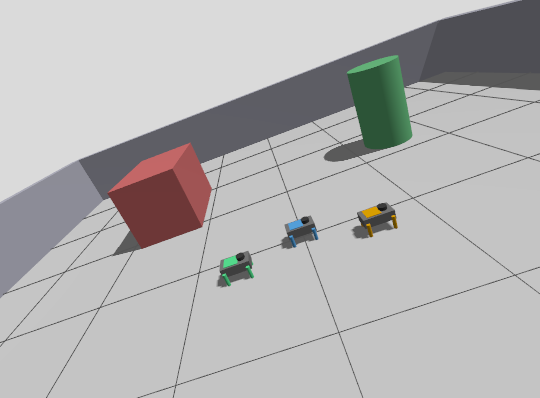
\includegraphics[width=\textwidth]{figuras/gazebo_fleet_3d.png}
        \caption{Escena 3D en Gazebo Harmonic (\texttt{room.sdf}) con R1 (naranja), R2 (azul) y R3 (verde).}
        \label{fig:gazebo_fleet_3d}
    \end{subfigure}
    \hfill
    \begin{subfigure}[b]{0.48\textwidth}
        \centering
        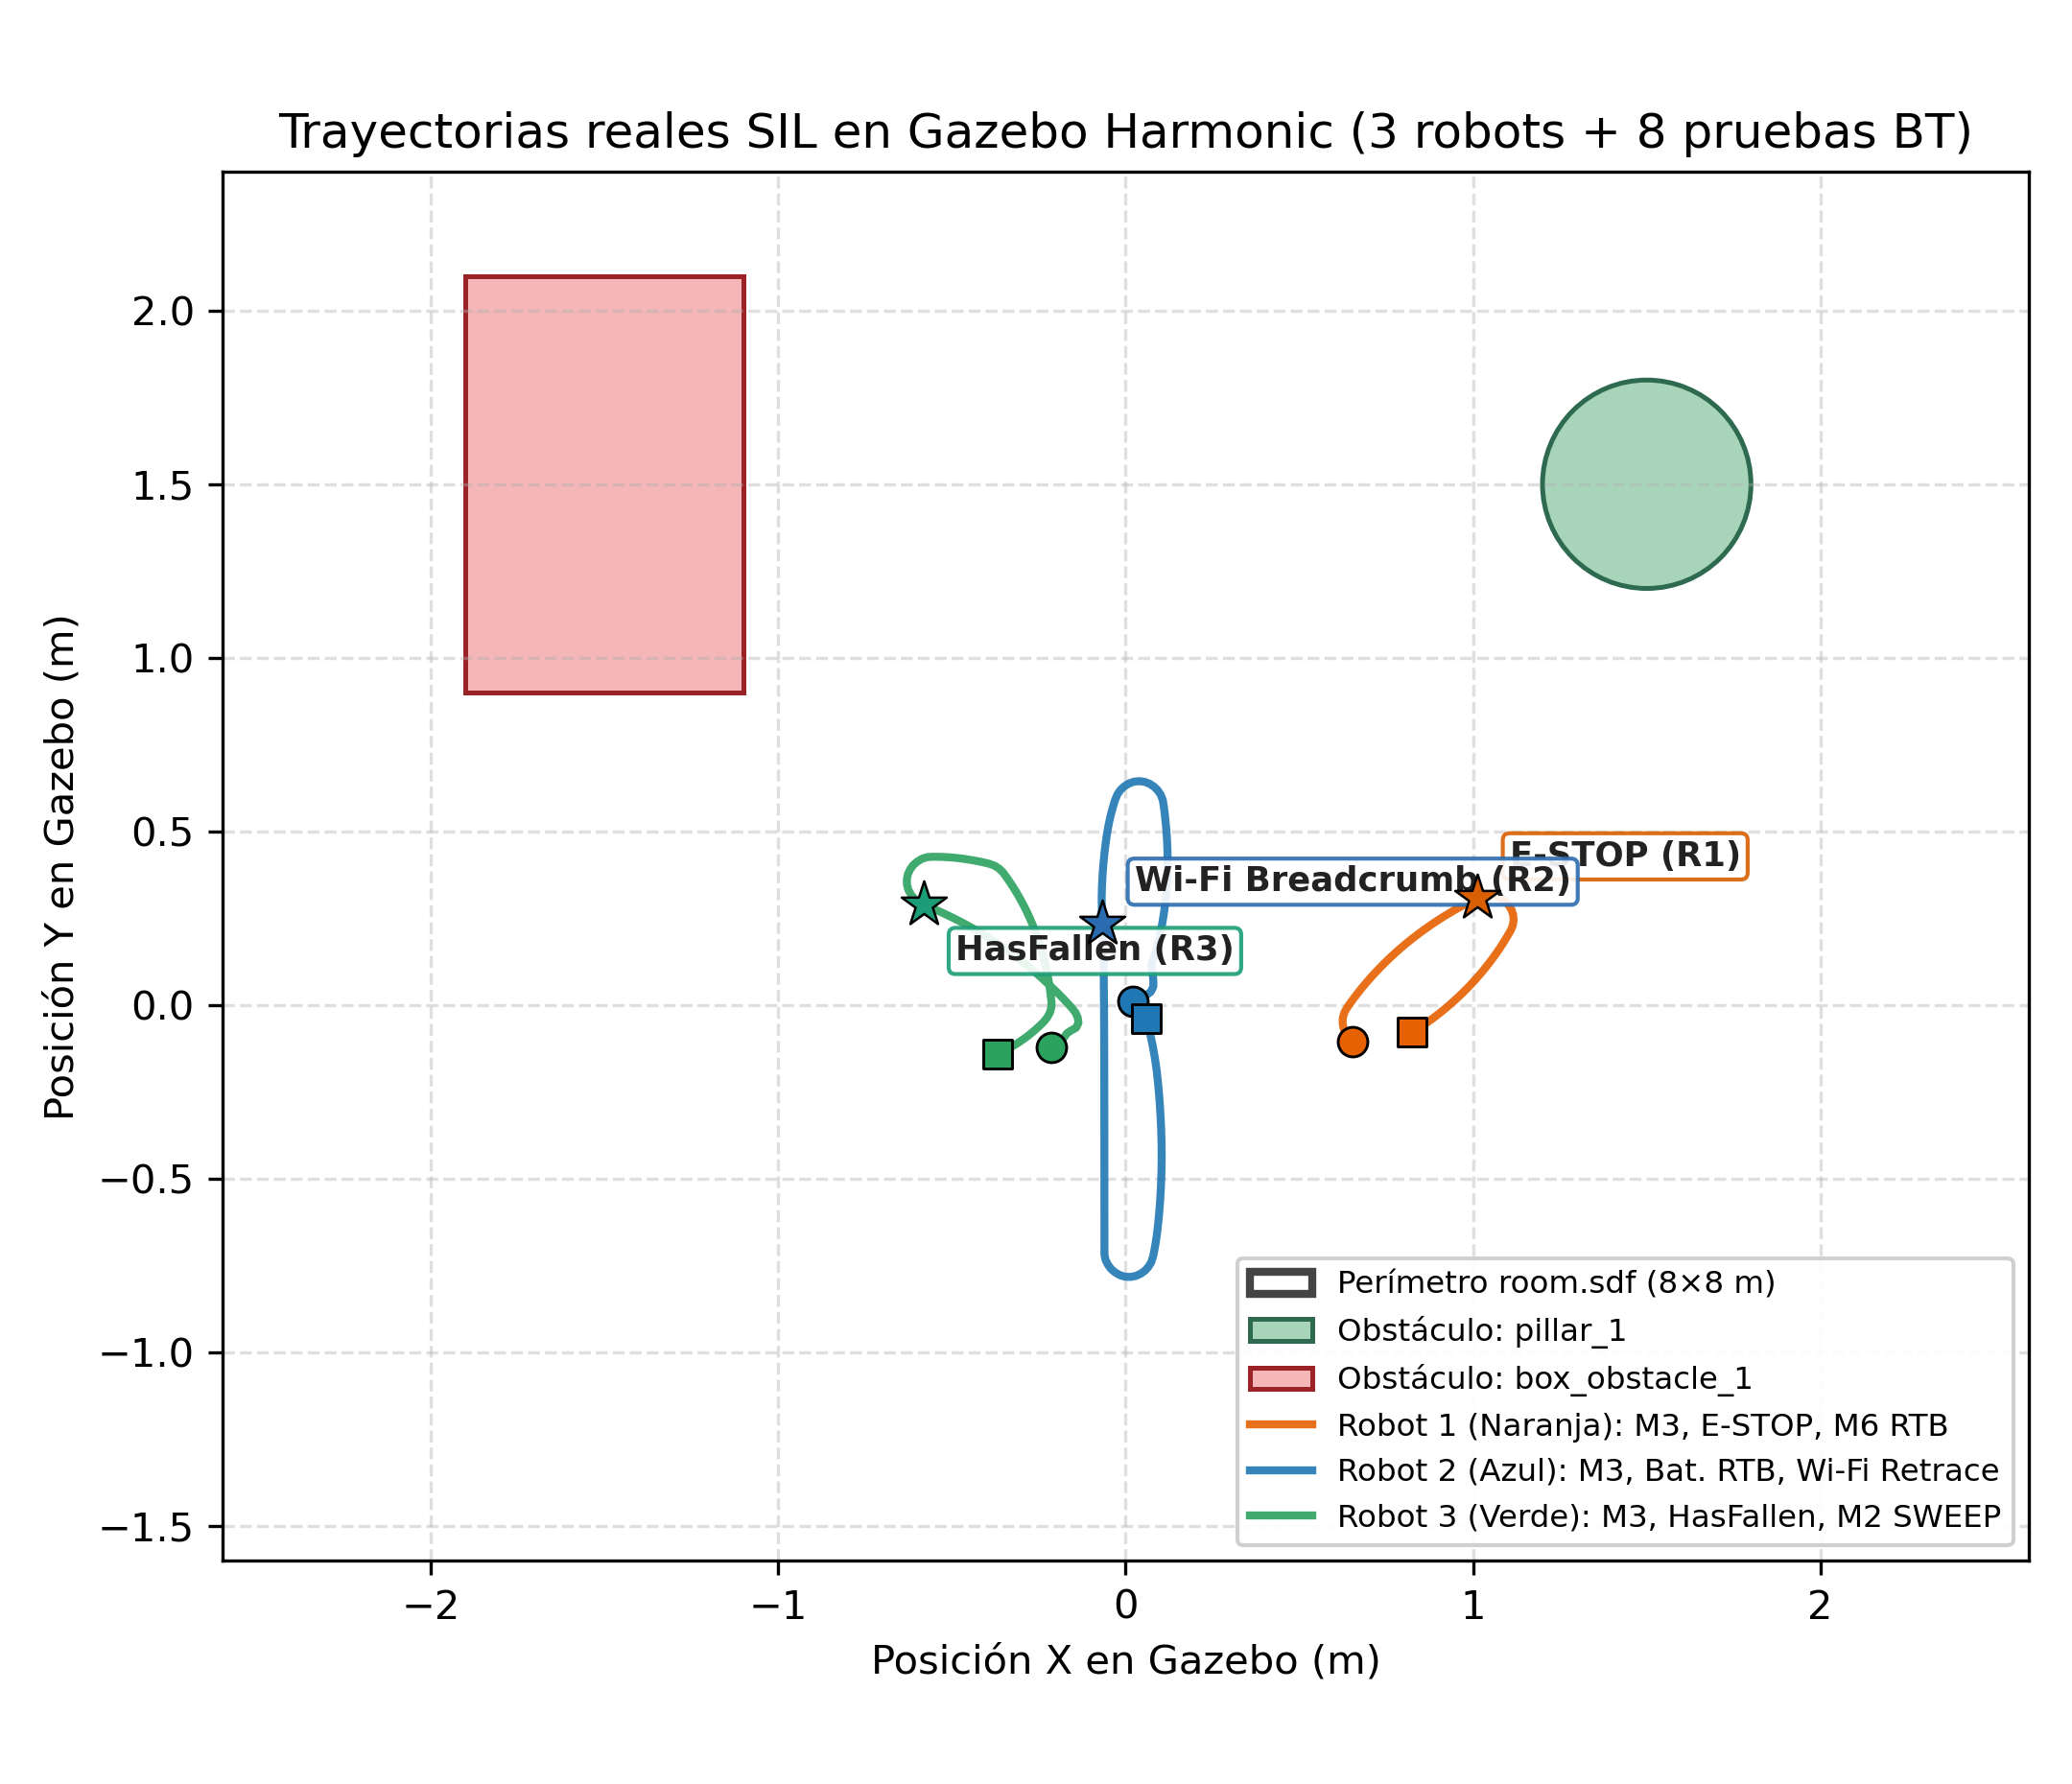
\includegraphics[width=\textwidth]{figuras/sil_trajectories_gazebo.png}
        \caption{Trayectorias reales de odometría y eventos de contingencia durante las 8 pruebas BT.}
        \label{fig:sil_trajectories}
    \end{subfigure}
    \caption{Validación SIL multi-robot sobre Gazebo Harmonic: entorno físico 3D y trayectorias registradas en bucle cerrado.}
    \label{fig:validacion_sil_gazebo}
\end{figure}

\begin{table}[htbp]
    \centering
    \caption{Resultados de la batería automatizada de validación SIL de los Behavior Trees sobre Gazebo Harmonic (3 robots concurrentes).}
    \label{tab:resultados_sil_gazebo}
    \footnotesize
    \begin{tabular}{clcl}
        \toprule
        \textbf{\#} & \textbf{Escenario / Rama evaluada} & \textbf{Estado} & \textbf{Métrica observada en Gazebo} \\
        \midrule
        1 & Conectividad Gazebo $\leftrightarrow$ 3 BTs & \textbf{PASS} & Odometría activa en R1, R2 y R3 \\
        2 & Rama 4: M3 \texttt{GOTO\_POINT} concurrente & \textbf{PASS} & $t=4.9$\,s; error $0.24$--$0.30$\,m \\
        3 & Rama 1: Preempción \texttt{E-STOP} (R1) & \textbf{PASS} & Alerta y parada (\texttt{cmd\_vel}=0) \\
        4 & Rama 1: Vuelco IMU \texttt{HasFallen} $>60^\circ$ (R3) & \textbf{PASS} & Alerta \textit{Rollover/Fallen} y parada \\
        5 & Rama 2: Batería crítica ($10\%$) $\rightarrow$ RTB (R2) & \textbf{PASS} & Retorno al dock ($0.58 \rightarrow 0.25$\,m) \\
        6 & Rama 3: Pérdida Wi-Fi $\rightarrow$ \textit{Retrace} (R2) & \textbf{PASS} & Alejado $0.46$\,m $\rightarrow$ retorno $0.32$\,m \\
        7 & Rama 4: M2 \texttt{SWEEP\_AREA} (3 waypoints, R3) & \textbf{PASS} & $t=10.8$\,s; 3/3 waypoints \\
        8 & Rama 4: M6 \texttt{RTB} explícito + logs Groot2 & \textbf{PASS} & \texttt{START\_RTB}/\texttt{DOCKED} + 3 \texttt{.btlog} \\
        \bottomrule
    \end{tabular}
\end{table}

La Figura~\ref{fig:validacion_sil_gazebo} muestra el entorno 3D en Gazebo Harmonic junto con las trayectorias reales registradas por los tres robots durante la ejecución completa de la batería de pruebas.

\subsection{Incidencias detectadas y corregidas durante la validación SIL}

La ejecución sistemática en Gazebo con el watchdog real de comunicaciones activo (\texttt{simulate\_heartbeat:=false}) permitió detectar y corregir dos defectos relevantes antes del despliegue físico:

\begin{itemize}
    \item \textbf{Reactividad de la Rama~3 (\texttt{Branch3\_Wifi}):} inicialmente modelada como un \texttt{Sequence} plano, impedía abortar el periodo de gracia de 5\,s si el enlace Wi-Fi se recuperaba antes de vencer. Asimismo, cambiar el nodo directamente a \texttt{ReactiveSequence} reiniciaba \texttt{Wait\_WifiGracePeriod} en cada \textit{tick}. La solución definitiva encapsula \texttt{Wait} y \texttt{NavigateToPose} dentro de un subnodo \texttt{Sequence} bajo un \texttt{ReactiveSequence}, logrando cancelación instantánea al recuperar el \textit{heartbeat} sin reiniciar la temporización.
    \item \textbf{Fijación de la miga de pan Wi-Fi (\texttt{last\_known\_wifi\_pose}):} actualizar esta pose desde el callback de odometría durante la ventana de timeout desplazaba el punto seguro hacia la zona sin cobertura. Se vinculó su actualización estrictamente a la recepción efectiva de paquetes en \texttt{/heartbeat}, garantizando que el robot retrocede al último punto con conectividad real confirmada.
\end{itemize}
